\chapter{Estudio del Prblema Singular}

    En Este capitulo se van a aplicar las herramientas desarrolladas en el capitulo anterior al estudio del espectro de un operador singular

\section{El Operador Singular}

Como trabajo de tesis se propondra aplicar los metodos desarrollados en el capitulo anterior al operador diferencial (\ref{operador}).

\begin{equation}
\begin{array}{c}
    A \phi (x) = - \partial ^2 _x  \phi(x) - \frac{\alpha}{x} \phi(x) \\
    \alpha > 0 \\ 
    \phi(0) = \phi(L) = 0 
\end{array}
\label{operador}
\end{equation}

Para eso voy a resolver la ecuación de autovalores (\ref{eq.aut.sin}).

\begin{equation}
\begin{array}{c}
    A [ \phi (x) ] =  \omega ^2 \phi (x) \\ 
    \omega \ \in \ \mathfrak{R}
\end{array}
\label{eq.aut.sin}
\end{equation}

La cual posee soluciones LI $ y_1 $ y $ y_2 $ dadas por :

\begin{equation}
    \phi (x) = 
    \underbrace{
    C[1] \ e ^{-i \omega x} \ x \ F _{1} ^{1} (1+\frac{i \alpha}{2 \omega},2,2 i \omega x) } _ {y_1}
    + \underbrace{C[2] \ e^{-i \omega x } \ x \ U (1+\frac{i \alpha}{2 \omega},2,2 i \omega x) } _{y_2}
\end{equation}

Donde $F _1 ^1(a,b,z)$ y $ U(a,b,z)$ son las soluciones LI de la ecuacion hypergeometrica (\ref{eq:hyper})

\begin{equation}
    z \ \partial ^2 _z \ \psi (a,b,z) + (b-z) \
    \partial _z \psi (a,b,z)
    -a \ \psi (a,b,z) = 0
\label{eq:hyper}
\end{equation}

Aplciando la condicion de contorno $\phi (0) = 0$, debido a que $U (1+\frac{i \alpha}{2 \omega},2,0) \rightarrow \infty $ se obtiene $C[2]=0$


Los autovalores entonces están dados por los ceros de $y _1 (L) = 0 $, donde la única función que se anula en el producto es  $F _1 ^1 (1+\frac{i \alpha}{2 \omega},2,2 i \omega x) $, los autovalores estarán caracterizados por  $F _1 ^1$, en la figura (\ref{fig:funcion}) se puede ver su comportamiento en funcion de $\omega$ para  $\alpha=1, \ L=1$.

\begin{figure}
\centering
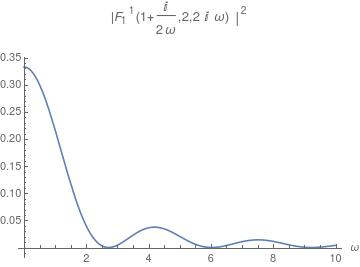
\includegraphics[scale=0.7]{Funcion.jpg}
\caption{En esta imagen se puede ver el comportamiento de los ceros de función $F _1 ^1$, para $\alpha=1$ y $L=1$}
\label{fig:funcion}
\end{figure}

A partir de ahora en vez de trabajar con la función hypergeometrica, voy a trabajar con su aproximación dada por (\ref{eq.aprox}) la cual tiene validez para $|z| \rightarrow \infty$ . (COMO CITO EL ABRA)

\begin{equation}
    F _1 ^1 (a,b,z) = \Gamma (b) 
    \left(
    \frac{e^z z ^{a-b} }{\Gamma(a)} * A_1 + \frac{(-z) ^{ -a}}{ \Gamma(b-a)} 
    * A_2
    \right)
\label{eq.aprox}
\end{equation}

Donde $A_1$ y $A_2$ son correcciones asintóticas, que voy a tomar como 1, en el apéndice 1 se demuestra que no contribuyen a la estructura de los polos, al orden que estoy calculando, si hay que tenerlos en cuenta para calcular los polos mas halla de donde se calcularon en esta tesis.

Definiendo las variables adimensionales $\mu = \omega L$  y $\beta = \alpha L $ y reemplazando los valores correspondientes en la ecuación (\ref{eq.aprox}) obtengo. 

\begin{equation}
    F _1 ^1 (1+ i \frac{  \beta}{2 \mu} ,2 ,2 i \beta ) = 
    \frac{e ^{- \frac{\pi}{4} \frac{\beta}{\mu} } }{2 \mu}
    \left(
    \frac{e ^{i (\frac{\beta}{2 mu} Ln(2 \mu) - \pi/2+ 2 \mu))}}{\Gamma(1+\frac{i \beta}{2 \mu})} + 
    \frac{e ^{- i (\frac{\beta}{2 mu} Ln(2 \mu) - \pi/2 ))}}{\Gamma(1-\frac{i \beta}{2 \mu})}
    \right)
\label{eq.completa}
\end{equation}




La cual queda expresada como un producto de dos funciones, una parte que se anula y una parte que no.

Para obtener los autovalores voy a solo ocuparme de la parte que se anula, la cual esta entre paréntesis.

\begin{equation}
    M (\mu) = 
    \frac{e ^{i (\frac{\beta}{2 \mu} Ln(2 \mu) - \pi/2+ 2 \mu))}}{\Gamma(1+\frac{i \beta}{2 \mu})} + 
    \frac{e ^{- i (\frac{\beta}{2 \mu} Ln(2 \mu) - \pi/2 ))}}{\Gamma(1-\frac{i \beta}{2 \mu})}
\label{eq.aproxx}
\end{equation}

Para calcular los polos de $\zeta _A (s)$ voy a utilizar las técnicas desarrolladas en el capitulo anterior.

\section{Calculo Asintótico de los autovalores}

\section{Calculo Utilizando Variable Compleja}


Sabiendo que los autovalores de mi ecuación son todos reales, puedo expresar mi  $\zeta _A (s)$ como una integral en el plano complejo, y sabiendo que no presenta ningun otro polo, puedo deformarlo hasta que quede el camino dado por (\ref{fig:contorno}) tal como había echo antes


La función $\zeta _A (s)$ queda definida por la ecuación (CAPITULO ANTERIOR), donde $f(\omega)$ donde al igual que antes voy a usar la ecuación (\ref{eq.aproxx}) en vez de  (\ref{eq.completa}) ya que ambas poseen los mismos ceros. 

Cuando deforme el camino en la integral sobre los ejes verticales, voy a obtener un termino exponencialmente decreciente y uno decreciente, que se van a alternar dependiendo de si estoy arriba o abajo del eje real.

voy a tener que calcular $f'(\omega)$ y $f(\omega)$ para luego evaluar $\omega$ = $\pm i t$, donde t es el parámetro de integración .

Para evitar trabajar con todos los terminos de la expresion (\ref{eq.aproxx}) voy a renombrar distintas partes de la ecuacion segun:

\begin{equation}
\begin{array}{c}
    q = \frac{\alpha}{2 \beta} Log[2 \omega L] \\
    q' = \partial _\omega q \\
    p = 2 i \mu \\
    p' = \partial _\omega p \\
    \Gamma _{\pm} = \Gamma(1 \pm \frac{i \alpha}{2 \omega}) \\
    \psi ^{\pm} = \frac{1}{\Gamma _{\pm}} \partial _{\omega}  \Gamma _{\pm} \\
\end{array}
\end{equation}

Utilizando estas definiciones, mi ecuación (\ref{eq.aproxx}) queda:

\begin{equation}
    f(\omega) = - \frac{i e^{i(q+p)}}
    {\Gamma _{+}} +
    \frac{i e^{- i \ q}}
    {\Gamma _{-}}
\end{equation}

Luego calculando $\partial _{\omega} f(\omega)$ obtengo:

\begin{equation}
    f' = 
    e^ {i p}
    \underbrace
    {
    e ^{i q}
    \left(
    \frac{1}{\Gamma _{+}}  \partial _{\omega} (q+p)
    + i 
    \frac
    {\partial _{\omega} \Gamma _{+} }
    {\Gamma _{+} ^2}
    \right)    +
    e^ {-i q}
    \left(
    \frac{1}{\Gamma _{-}}  \partial _{\omega} q
    - i 
    \frac
    {\partial _{\omega} \Gamma _{-} }
    {\Gamma _{-} ^2}
    \right)
    } _{*}
\end{equation}

Donde todo el termino marcado con  $*$ cuando haga la sustitucion $\omega = \pm i t$ para hacer la integral sobre los ejes, van a converger $\forall \ t$ sin importar el eje.

El problema va a surgir cuando cuando quiera evaluar $e ^{i p}$, voy a obtener un termino exponencialmente creciente, dependiendo si el eje es -i, para eso, saco factor común $e ^{i p}$ en $f \ y \ f'$ cancelando el termino exponencialmente creciente y obteniendo una suma con un termino exponencialmente decreciente, obteniendo finalmente:

\begin{equation}
\begin{array}{c}
    \frac{f'}{f} = \frac{1}{i} 
    \left(
    q' - i 
    \frac
    {\partial _{\omega} \Gamma _{-} }
    {\Gamma _{-}}
    \right)
    \\
    Para \ \omega = i t 
\end{array}
\end{equation}
    
\begin{equation}
\begin{array}{c}
    \frac{f'}{f} = i 
    \left(
    q'+p' + i 
    \frac
    {\partial _{\omega} \Gamma _{+} }
    {\Gamma _{+}}
    \right)
    \\
    Para \ \omega = - i t 
\end{array}
\end{equation}
    
Donde en las ecuaciones de arriba, reemplazando las definicinoes de $q \ y \ p$ obtengo, respectivamente

\begin{equation}
\begin{array}{c}
    \frac{\alpha}{2 i \omega ^2}
    \left(
    1 - Log(2 \omega L ) + \psi (1-\frac{\alpha}{2 \beta \omega})
    \right) \\
    \frac{i \alpha}{2 \omega ^2}
    \left(
    1 - Log(2 \omega L ) + \psi  (1  + \frac{\alpha}{2 \beta \omega})
    \right) + 
    2 i L
\end{array}
\end{equation}

Reemplazando estos resultados en la integral obtengo 

\begin{equation}
\begin{array}{c}
    \zeta _A (s) = \\
     \frac{1}{2 \pi i} \int _{\infty} ^{1}
     \frac{i \alpha}{2 t^2}
     \left(
     1 - Log(2 L t) - \frac{i \pi}{2} + \psi (1-\frac{\alpha}{2 t})
     \right)
     t^{-2 s}
     e^{-i \pi s} \ 
     (i dt) + \\
     \frac{1}{2 \pi i} \int _1 ^{\infty}
     \frac{ \alpha}{2 i t^2}
     \left(
     \left(
     1 - Log(2 L t) - \frac{i \pi}{2} + \psi (1-\frac{\alpha}{2 t}) 
     \right)
     + 2 i L
     \right)
     t^{-2 s}
     e^{i \pi s}
     (-i dt)
     
\end{array}
\end{equation}

Donde antes de reacomodar los terminos puedo calcular el termino que contiene $2iL$ el cual es la potencia mas alta de $t$ para obtener: 

\begin{equation}
    \frac{1}{2 \pi i }
    \int _1 ^{\infty}
    2 i L
    e^{i \pi s}
    t ^{-2 s}
    (-i dt) =  
    \frac{L e^{i \pi s} }{2 \pi i} \frac{1}{s-1/2   }
\end{equation}

Ningún otro termino aportará a este polo, entonces el residuo en $s= 1/2$ es:

\begin{equation}
    Res (s=1/2) = \frac{L}{2 \pi}
\end{equation}

Que se corresponde con el calculado con el método anterior.

Una vez calculado este termino, puedo reorganizar el resto de la integral como:

\begin{equation}
\begin{array}{c}
    - \frac{\alpha}{2 \pi} \ sin[\pi s]
    \int _1 ^{\infty}
    t ^{-2 s-s} 
    \left(
    1 - Log[2Lt] + \psi (1- \frac{\alpha}{2t})
    \right) dt - 
    \frac{\alpha}{4} 
    Cos[\pi s]
    \int _1 ^{\infty} t^{-2s-s} dt
\end{array}
\end{equation}

Donde todos los términos son calculables analíticamente, excepto el que esta multiplicado por $\psi$, para lo cual utilizo el desarrollo de $\psi$ en $t \rightarrow \infty$:

\begin{equation}
    \psi(1-\frac{\alpha}{2 t}) \approx 
    -\gamma + O(\frac{1}{t})
\end{equation}

Realizando todas las integrales la funcion $zeta _A (s)$ a este orden queda determinada por:  

\begin{equation}
\begin{array}{c}
    \zeta (s) _{A} = 
    \frac{L e ^{i \pi s}}{2 \pi i} \frac{1}{s-1/2} 
    -\frac{\alpha Sin[\pi s]}{4 \pi} \frac{1}{s+1/2} \\
    \alpha 
    \frac{
    1+S Log(4)+2SLog[L]+Log[2L]
    }
    {8 \pi} \frac{sin(\pi s)}{(s+1/2) ^2}  \\
    \frac{\gamma \alpha Sin[\pi s]}{4 \pi } \frac{1}{s+1/2} 
    \frac{\alpha cos(\pi s) }{8 \pi}  \frac{1}{s+1/2}  \\
\end{array}
\end{equation}

Donde el siguiente termino en el desarrollo de $psi$ contribuirá al residuo en $s = -3/2$

Para calcular el residuo en $s=-1/2$ desarrollo todo en Serie de Laurent alrededor de ese punto obteniendo.

\begin{equation}
    - \frac{\alpha}{8 \pi} \frac{1}{(s+1/2)^2} + 
    \alpha \frac{1-\gamma -Log[2 L]}{4 \pi} \frac{1}{s+1/2} + \ Regular
\label{eq.desarrollo}
\end{equation}

Donde se puede ver que el residuo, y la contribución al polo cuadrático en $s=-1/2$ coinciden con las calculadas anteriormente.

Una aclaracion importante es que el termino $Log[2 L ]$ es correcto dimensionalmente, ya que proviene de evaluar la integral $\int _1 ^\infty
 Log[2 L \omega] \ d \omega$

\section{Cálculo de la energía de vacío}

La energía de vacío queda determinada por la ecuación 

\begin{equation}
    E _0 = \frac{\hbar}{2}  
    \zeta (s)  |  _{- \frac{1}{2}}
\end{equation}

$\zeta (s)$ ya está desarrollada alrededor de $s=-1/2$ en (\ref{eq.desarrollo}), queda desarrollar $(E_c) ^{2s+1} $ alrededor de $s=-1/2$ quedando.

\begin{equation}
    E _c \approx 
    1 + 2 Log[E_c] (s + 1/2) +
    2 Log[E_c] ^2 (s+1/2) ^2 + 
    O (s+1/2)^3
\end{equation}

Entonces la energía de vació queda determinada por:

\begin{equation}
    E _0 =
    \left(
    \frac{1}{(s+1/2)^2} 
    \left(
    \frac{- \alpha}{8 \pi}
    \right)+
    \frac{
    \alpha(1 -\gamma-Log[2L]) - 
    \alpha Log[E_c] 
    }{4 \pi (s+1/2)} 
     + Regular
    \right) | _{s=-1/2}
\end{equation}








